\documentclass[twoside]{book}

% Packages required by doxygen
\usepackage{fixltx2e}
\usepackage{calc}
\usepackage{doxygen}
\usepackage[export]{adjustbox} % also loads graphicx
\usepackage{graphicx}
\usepackage[utf8]{inputenc}
\usepackage{makeidx}
\usepackage{multicol}
\usepackage{multirow}
\PassOptionsToPackage{warn}{textcomp}
\usepackage{textcomp}
\usepackage[nointegrals]{wasysym}
\usepackage[table]{xcolor}

% Font selection
\usepackage[T1]{fontenc}
\usepackage[scaled=.90]{helvet}
\usepackage{courier}
\usepackage{amssymb}
\usepackage{sectsty}
\renewcommand{\familydefault}{\sfdefault}
\allsectionsfont{%
  \fontseries{bc}\selectfont%
  \color{darkgray}%
}
\renewcommand{\DoxyLabelFont}{%
  \fontseries{bc}\selectfont%
  \color{darkgray}%
}
\newcommand{\+}{\discretionary{\mbox{\scriptsize$\hookleftarrow$}}{}{}}

% Page & text layout
\usepackage{geometry}
\geometry{%
  a4paper,%
  top=2.5cm,%
  bottom=2.5cm,%
  left=2.5cm,%
  right=2.5cm%
}
\tolerance=750
\hfuzz=15pt
\hbadness=750
\setlength{\emergencystretch}{15pt}
\setlength{\parindent}{0cm}
\setlength{\parskip}{3ex plus 2ex minus 2ex}
\makeatletter
\renewcommand{\paragraph}{%
  \@startsection{paragraph}{4}{0ex}{-1.0ex}{1.0ex}{%
    \normalfont\normalsize\bfseries\SS@parafont%
  }%
}
\renewcommand{\subparagraph}{%
  \@startsection{subparagraph}{5}{0ex}{-1.0ex}{1.0ex}{%
    \normalfont\normalsize\bfseries\SS@subparafont%
  }%
}
\makeatother

% Headers & footers
\usepackage{fancyhdr}
\pagestyle{fancyplain}
\fancyhead[LE]{\fancyplain{}{\bfseries\thepage}}
\fancyhead[CE]{\fancyplain{}{}}
\fancyhead[RE]{\fancyplain{}{\bfseries\leftmark}}
\fancyhead[LO]{\fancyplain{}{\bfseries\rightmark}}
\fancyhead[CO]{\fancyplain{}{}}
\fancyhead[RO]{\fancyplain{}{\bfseries\thepage}}
\fancyfoot[LE]{\fancyplain{}{}}
\fancyfoot[CE]{\fancyplain{}{}}
\fancyfoot[RE]{\fancyplain{}{\bfseries\scriptsize Generated by Doxygen }}
\fancyfoot[LO]{\fancyplain{}{\bfseries\scriptsize Generated by Doxygen }}
\fancyfoot[CO]{\fancyplain{}{}}
\fancyfoot[RO]{\fancyplain{}{}}
\renewcommand{\footrulewidth}{0.4pt}
\renewcommand{\chaptermark}[1]{%
  \markboth{#1}{}%
}
\renewcommand{\sectionmark}[1]{%
  \markright{\thesection\ #1}%
}

% Indices & bibliography
\usepackage{natbib}
\usepackage[titles]{tocloft}
\setcounter{tocdepth}{3}
\setcounter{secnumdepth}{5}
\makeindex

% Hyperlinks (required, but should be loaded last)
\usepackage{ifpdf}
\ifpdf
  \usepackage[pdftex,pagebackref=true]{hyperref}
\else
  \usepackage[ps2pdf,pagebackref=true]{hyperref}
\fi
\hypersetup{%
  colorlinks=true,%
  linkcolor=blue,%
  citecolor=blue,%
  unicode%
}

% Custom commands
\newcommand{\clearemptydoublepage}{%
  \newpage{\pagestyle{empty}\cleardoublepage}%
}

\usepackage{caption}
\captionsetup{labelsep=space,justification=centering,font={bf},singlelinecheck=off,skip=4pt,position=top}

%===== C O N T E N T S =====

\begin{document}

% Titlepage & ToC
\hypersetup{pageanchor=false,
             bookmarksnumbered=true,
             pdfencoding=unicode
            }
\pagenumbering{roman}
\begin{titlepage}
\vspace*{7cm}
\begin{center}%
{\Large Erriez Timestamp library for Arduino \\[1ex]\large 1.\+0.\+0 }\\
\vspace*{1cm}
{\large Generated by Doxygen 1.8.11}\\
\end{center}
\end{titlepage}
\clearemptydoublepage
\tableofcontents
\clearemptydoublepage
\pagenumbering{arabic}
\hypersetup{pageanchor=true}

%--- Begin generated contents ---
\chapter{Timestamp measuring library for Arduino}
\label{index}\hypertarget{index}{}\href{https://travis-ci.org/Erriez/ErriezTimestamp}{\tt }

This is a timestamp library for Arduino to measure execution durations in microseconds or milliseconds resolution.



\subsection*{Hardware}

Any Arduino / E\+S\+P8266 board.

\subsection*{Library documentation}


\begin{DoxyItemize}
\item \href{https://Erriez.github.io/ErriezTimestamp}{\tt Doxygen online H\+T\+ML}
\item \href{https://github.com/Erriez/ErriezTimestamp/raw/gh-pages/latex/ErriezTimestamp.pdf}{\tt Doxygen P\+DF}
\end{DoxyItemize}

\subsection*{Examples}

Arduino I\+DE $\vert$ Examples $\vert$ Erriez \hyperlink{class_timestamp}{Timestamp}\+:


\begin{DoxyItemize}
\item \href{https://github.com/Erriez/ErriezTimestamp/blob/master/examples/Microseconds/Microseconds.ino}{\tt Microseconds}
\item \href{https://github.com/Erriez/ErriezTimestamp/blob/master/examples/Milliseconds/Milliseconds.ino}{\tt Milliseconds}
\end{DoxyItemize}

\#\# Example output \hyperlink{class_timestamp}{Timestamp} $\vert$ Microseconds 
\begin{DoxyCode}
1 Timestamp with microseconds resolution example
2 
3 Printing this message takes: 768us
4 And this message takes: 2044us
5 delayMicroseconds(15) duration: 20us
6 analogRead() duration: 212us
7 digitalRead() duration: 4us
\end{DoxyCode}


\#\# Example output \hyperlink{class_timestamp}{Timestamp} $\vert$ Milliseconds 
\begin{DoxyCode}
1 Timestamp with milliseconds resolution example
2 
3 delay(15) takes:
4 15ms
5 14ms
6 16ms
7 15ms
8 15ms
9 16ms
10 14ms
11 15ms
12 16ms
13 15ms
\end{DoxyCode}


\subsection*{Usage}

\subsubsection*{Initialization}

Add include file\+: 
\begin{DoxyCode}
1 \{c++\}
2 #include <ErriezTimestamp.h>
\end{DoxyCode}


Create timestamp object with microseconds resolution\+: 
\begin{DoxyCode}
1 \{c++\}
2 TimestampMicros timestamp;
\end{DoxyCode}


Create timestamp object with milliseconds resolution\+: 
\begin{DoxyCode}
1 \{c++\}
2 TimestampMillis timestamp;
\end{DoxyCode}


\#\#\# Single measurement 
\begin{DoxyCode}
1 \{c++\}
2 unsigned long duration;
3 
4 // Start measurement
5 timestamp.start();
6 // Do something
7 duration = timestamp.delta();
8 
9 // Start new measurement
10 timestamp.start();
11 // Do something
12 duration = timestamp.delta();
\end{DoxyCode}


\#\#\# Multiple measurements 
\begin{DoxyCode}
1 \{c++\}
2 // Start timestamp
3 timestamp.start();
4 // Do something and print timstamp
5 timestamp.print();
6 
7 // Do something and print timestamp without calling start()
8 timestamp.print();
\end{DoxyCode}


\subsection*{Constraints}

\hyperlink{class_timestamp_micros}{Timestamp\+Micros} uses the function {\ttfamily micros()}. \hyperlink{class_timestamp_millis}{Timestamp\+Millis} uses the function millis().

Please refer to the description of these functions for the maximum possible duration and minimum resolution\+:


\begin{DoxyItemize}
\item \href{https://www.arduino.cc/reference/en/language/functions/time/micros/}{\tt https\+://www.\+arduino.\+cc/reference/en/language/functions/time/micros/}
\item \href{https://www.arduino.cc/reference/en/language/functions/time/millis/}{\tt https\+://www.\+arduino.\+cc/reference/en/language/functions/time/millis/}
\end{DoxyItemize}

The micro seconds timestamp functions have small overhead on low-\/end microcontrollers. For example calling {\ttfamily start()} and {\ttfamily delta} may result in it may take 4..8us deviation on an Arduino U\+NO. This is overhead is negligible on targets with a higher C\+PU clock such as the E\+S\+P8266.

\subsection*{Library installation}

Please refer to the \href{https://github.com/Erriez/ErriezArduinoLibrariesAndSketches/wiki}{\tt Wiki} page.

\subsection*{Other Arduino Libraries and Sketches from Erriez}


\begin{DoxyItemize}
\item \href{https://github.com/Erriez/ErriezArduinoLibrariesAndSketches}{\tt Erriez Libraries and Sketches} 
\end{DoxyItemize}
\chapter{Hierarchical Index}
\section{Class Hierarchy}
This inheritance list is sorted roughly, but not completely, alphabetically\+:\begin{DoxyCompactList}
\item \contentsline{section}{Timestamp}{\pageref{class_timestamp}}{}
\begin{DoxyCompactList}
\item \contentsline{section}{Timestamp\+Micros}{\pageref{class_timestamp_micros}}{}
\item \contentsline{section}{Timestamp\+Millis}{\pageref{class_timestamp_millis}}{}
\end{DoxyCompactList}
\end{DoxyCompactList}

\chapter{Class Index}
\section{Class List}
Here are the classes, structs, unions and interfaces with brief descriptions\+:\begin{DoxyCompactList}
\item\contentsline{section}{\hyperlink{class_timestamp}{Timestamp} \\*Timstamp class }{\pageref{class_timestamp}}{}
\item\contentsline{section}{\hyperlink{class_timestamp_micros}{Timestamp\+Micros} \\*\hyperlink{class_timestamp_micros}{Timestamp\+Micros} class derived from \hyperlink{class_timestamp}{Timestamp} }{\pageref{class_timestamp_micros}}{}
\item\contentsline{section}{\hyperlink{class_timestamp_millis}{Timestamp\+Millis} \\*\hyperlink{class_timestamp_millis}{Timestamp\+Millis} class derived from \hyperlink{class_timestamp}{Timestamp} }{\pageref{class_timestamp_millis}}{}
\end{DoxyCompactList}

\chapter{File Index}
\section{File List}
Here is a list of all documented files with brief descriptions\+:\begin{DoxyCompactList}
\item\contentsline{section}{\hyperlink{_timestamp_8cpp}{Timestamp.\+cpp} \\*\hyperlink{class_timestamp}{Timestamp} library for Arduino }{\pageref{_timestamp_8cpp}}{}
\item\contentsline{section}{\hyperlink{_timestamp_8h}{Timestamp.\+h} \\*\hyperlink{class_timestamp}{Timestamp} library for Arduino }{\pageref{_timestamp_8h}}{}
\end{DoxyCompactList}

\chapter{Class Documentation}
\hypertarget{class_timestamp}{}\section{Timestamp Class Reference}
\label{class_timestamp}\index{Timestamp@{Timestamp}}


Timstamp class.  




{\ttfamily \#include $<$Erriez\+Timestamp.\+h$>$}

Inheritance diagram for Timestamp\+:\begin{figure}[H]
\begin{center}
\leavevmode
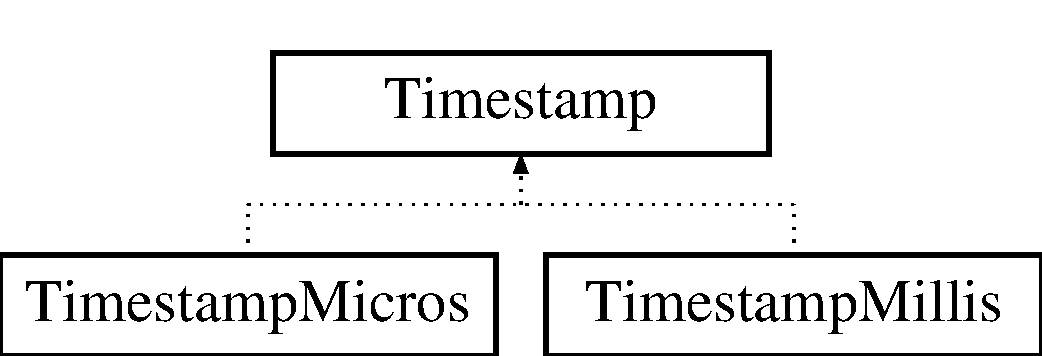
\includegraphics[height=2.000000cm]{class_timestamp}
\end{center}
\end{figure}
\subsection*{Public Member Functions}
\begin{DoxyCompactItemize}
\item 
\hyperlink{class_timestamp_a2e610487ef16d9d5a8d6dc8ad457a3e7}{Timestamp} ()\hypertarget{class_timestamp_a2e610487ef16d9d5a8d6dc8ad457a3e7}{}\label{class_timestamp_a2e610487ef16d9d5a8d6dc8ad457a3e7}

\begin{DoxyCompactList}\small\item\em \hyperlink{class_timestamp}{Timestamp} constructor. \end{DoxyCompactList}\item 
virtual void \hyperlink{class_timestamp_a4aa0acbd36d3e022b3e7e43bc4d9b5db}{start} ()=0\hypertarget{class_timestamp_a4aa0acbd36d3e022b3e7e43bc4d9b5db}{}\label{class_timestamp_a4aa0acbd36d3e022b3e7e43bc4d9b5db}

\begin{DoxyCompactList}\small\item\em Derived class must implement \hyperlink{class_timestamp_a4aa0acbd36d3e022b3e7e43bc4d9b5db}{start()} \end{DoxyCompactList}\item 
virtual unsigned long \hyperlink{class_timestamp_a47e8cbc581a8af32201e7b1088733043}{end} ()=0\hypertarget{class_timestamp_a47e8cbc581a8af32201e7b1088733043}{}\label{class_timestamp_a47e8cbc581a8af32201e7b1088733043}

\begin{DoxyCompactList}\small\item\em Derived class must implement \hyperlink{class_timestamp_a47e8cbc581a8af32201e7b1088733043}{end()} \end{DoxyCompactList}\item 
virtual unsigned long \hyperlink{class_timestamp_a351537b95385937a004ab32b6b3743f7}{print} ()=0\hypertarget{class_timestamp_a351537b95385937a004ab32b6b3743f7}{}\label{class_timestamp_a351537b95385937a004ab32b6b3743f7}

\begin{DoxyCompactList}\small\item\em Derived class must implement \hyperlink{class_timestamp_a351537b95385937a004ab32b6b3743f7}{print()} \end{DoxyCompactList}\end{DoxyCompactItemize}
\subsection*{Protected Attributes}
\begin{DoxyCompactItemize}
\item 
unsigned long \hyperlink{class_timestamp_a9adad295553fbb0b4479e04ac4f506a1}{\+\_\+timestamp\+Start}\hypertarget{class_timestamp_a9adad295553fbb0b4479e04ac4f506a1}{}\label{class_timestamp_a9adad295553fbb0b4479e04ac4f506a1}

\begin{DoxyCompactList}\small\item\em \hyperlink{class_timestamp}{Timestamp} at the beginning of a measurement. \end{DoxyCompactList}\end{DoxyCompactItemize}


\subsection{Detailed Description}
Timstamp class. 

Definition at line 42 of file Erriez\+Timestamp.\+h.



The documentation for this class was generated from the following files\+:\begin{DoxyCompactItemize}
\item 
\hyperlink{_erriez_timestamp_8h}{Erriez\+Timestamp.\+h}\item 
\hyperlink{_erriez_timestamp_8cpp}{Erriez\+Timestamp.\+cpp}\end{DoxyCompactItemize}

\hypertarget{class_timestamp_micros}{}\section{Timestamp\+Micros Class Reference}
\label{class_timestamp_micros}\index{Timestamp\+Micros@{Timestamp\+Micros}}


\hyperlink{class_timestamp_micros}{Timestamp\+Micros} class derived from \hyperlink{class_timestamp}{Timestamp}.  




{\ttfamily \#include $<$Erriez\+Timestamp.\+h$>$}

Inheritance diagram for Timestamp\+Micros\+:\begin{figure}[H]
\begin{center}
\leavevmode
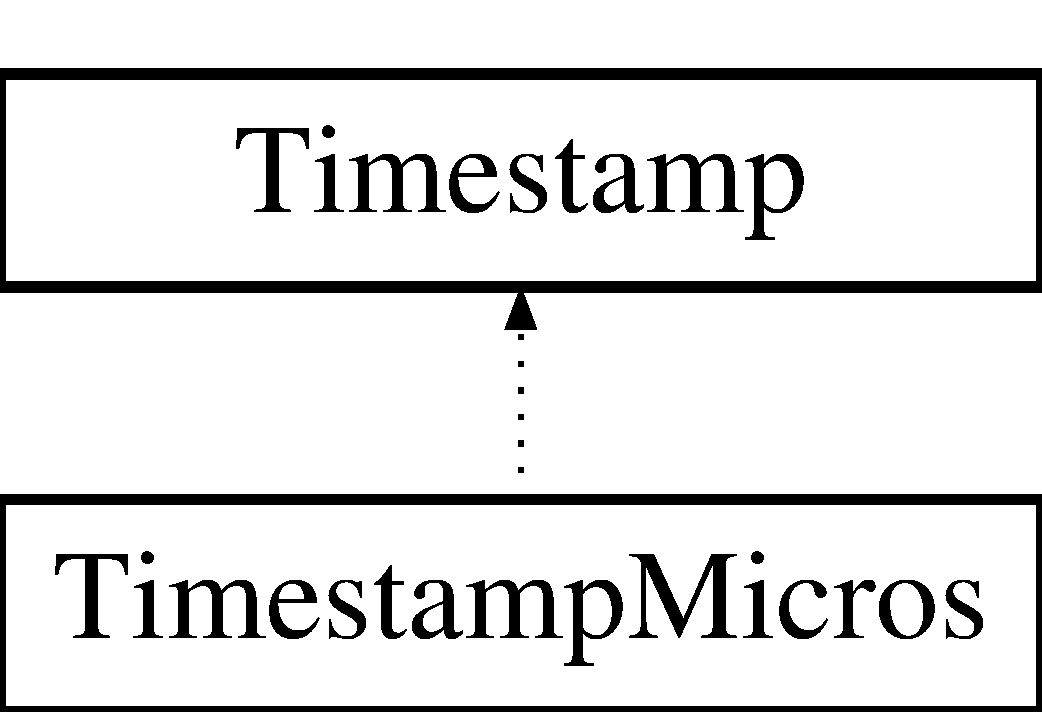
\includegraphics[height=2.000000cm]{class_timestamp_micros}
\end{center}
\end{figure}
\subsection*{Public Member Functions}
\begin{DoxyCompactItemize}
\item 
void \hyperlink{class_timestamp_micros_a847c7bc584b217cc901b22c1e08b013e}{start} () override\hypertarget{class_timestamp_micros_a847c7bc584b217cc901b22c1e08b013e}{}\label{class_timestamp_micros_a847c7bc584b217cc901b22c1e08b013e}

\begin{DoxyCompactList}\small\item\em Start measurement in microseconds. \end{DoxyCompactList}\item 
unsigned long \hyperlink{class_timestamp_micros_ae0489e7ea01e5a726b23ee3243868e92}{delta} () override
\begin{DoxyCompactList}\small\item\em End measurement. \end{DoxyCompactList}\item 
void \hyperlink{class_timestamp_micros_afb2a63d2cd3d42b66186462c2e79b5d1}{print} () override
\begin{DoxyCompactList}\small\item\em Print measurement in microseconds. \end{DoxyCompactList}\end{DoxyCompactItemize}


\subsection{Detailed Description}
\hyperlink{class_timestamp_micros}{Timestamp\+Micros} class derived from \hyperlink{class_timestamp}{Timestamp}. 

Definition at line 57 of file Erriez\+Timestamp.\+h.



\subsection{Member Function Documentation}
\index{Timestamp\+Micros@{Timestamp\+Micros}!delta@{delta}}
\index{delta@{delta}!Timestamp\+Micros@{Timestamp\+Micros}}
\subsubsection[{\texorpdfstring{delta() override}{delta() override}}]{\setlength{\rightskip}{0pt plus 5cm}unsigned long Timestamp\+Micros\+::delta (
\begin{DoxyParamCaption}
{}
\end{DoxyParamCaption}
)\hspace{0.3cm}{\ttfamily [override]}, {\ttfamily [virtual]}}\hypertarget{class_timestamp_micros_ae0489e7ea01e5a726b23ee3243868e92}{}\label{class_timestamp_micros_ae0489e7ea01e5a726b23ee3243868e92}


End measurement. 

\begin{DoxyReturn}{Returns}
Duration in micro seconds 
\end{DoxyReturn}


Implements \hyperlink{class_timestamp_afa237f41af2043b2f5d6e0733d595c21}{Timestamp}.



Definition at line 58 of file Erriez\+Timestamp.\+cpp.

\index{Timestamp\+Micros@{Timestamp\+Micros}!print@{print}}
\index{print@{print}!Timestamp\+Micros@{Timestamp\+Micros}}
\subsubsection[{\texorpdfstring{print() override}{print() override}}]{\setlength{\rightskip}{0pt plus 5cm}void Timestamp\+Micros\+::print (
\begin{DoxyParamCaption}
{}
\end{DoxyParamCaption}
)\hspace{0.3cm}{\ttfamily [override]}, {\ttfamily [virtual]}}\hypertarget{class_timestamp_micros_afb2a63d2cd3d42b66186462c2e79b5d1}{}\label{class_timestamp_micros_afb2a63d2cd3d42b66186462c2e79b5d1}


Print measurement in microseconds. 

Print millis() -\/ start time and restart measurement \begin{DoxyReturn}{Returns}
Duration in microseconds 
\end{DoxyReturn}


Implements \hyperlink{class_timestamp_a62b55270dae36ad337c87ae30eeb2fb9}{Timestamp}.



Definition at line 70 of file Erriez\+Timestamp.\+cpp.



The documentation for this class was generated from the following files\+:\begin{DoxyCompactItemize}
\item 
\hyperlink{_erriez_timestamp_8h}{Erriez\+Timestamp.\+h}\item 
\hyperlink{_erriez_timestamp_8cpp}{Erriez\+Timestamp.\+cpp}\end{DoxyCompactItemize}

\hypertarget{class_timestamp_millis}{}\section{Timestamp\+Millis Class Reference}
\label{class_timestamp_millis}\index{Timestamp\+Millis@{Timestamp\+Millis}}


\hyperlink{class_timestamp_millis}{Timestamp\+Millis} class derived from \hyperlink{class_timestamp}{Timestamp}.  




{\ttfamily \#include $<$Timestamp.\+h$>$}

Inheritance diagram for Timestamp\+Millis\+:\begin{figure}[H]
\begin{center}
\leavevmode
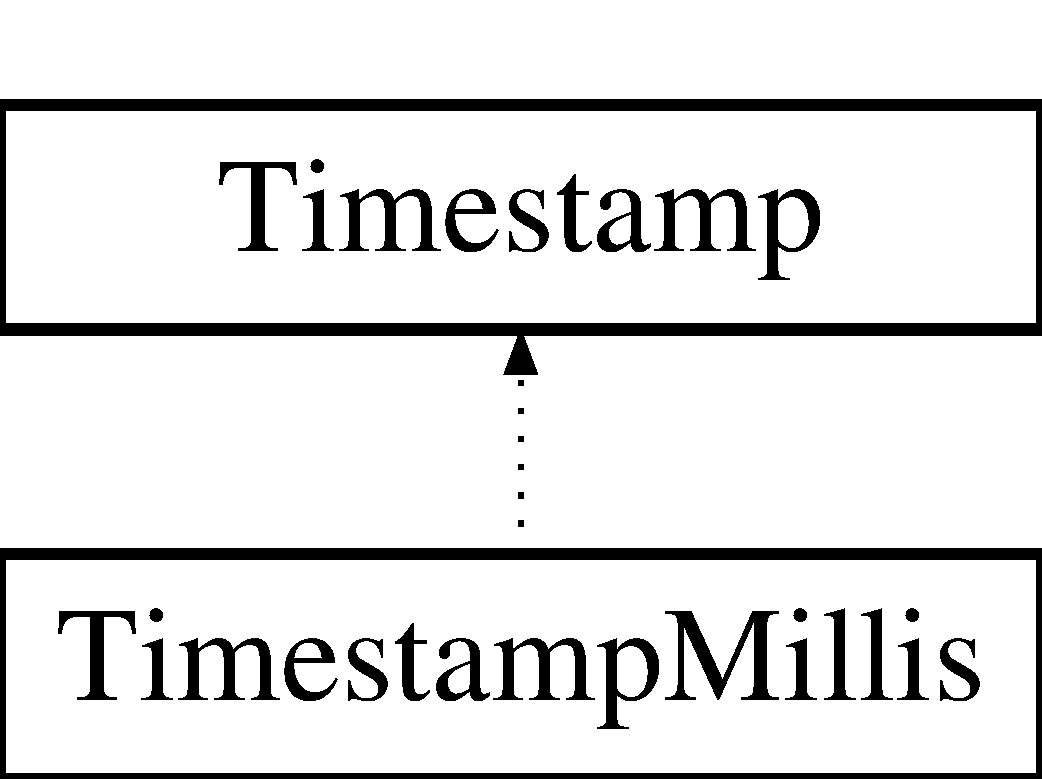
\includegraphics[height=2.000000cm]{class_timestamp_millis}
\end{center}
\end{figure}
\subsection*{Public Member Functions}
\begin{DoxyCompactItemize}
\item 
void \hyperlink{class_timestamp_millis_a4865760b8d19a2cff0b230c8bf0123d2}{start} () override\hypertarget{class_timestamp_millis_a4865760b8d19a2cff0b230c8bf0123d2}{}\label{class_timestamp_millis_a4865760b8d19a2cff0b230c8bf0123d2}

\begin{DoxyCompactList}\small\item\em Start measurement in milliseconds. \end{DoxyCompactList}\item 
unsigned long \hyperlink{class_timestamp_millis_ad0bd89a6d30c9ee317dded214dd3084c}{end} () override
\begin{DoxyCompactList}\small\item\em End measurement. \end{DoxyCompactList}\item 
unsigned long \hyperlink{class_timestamp_millis_a4994e32cdd53388cbb550d467ddbd6f9}{print} () override
\begin{DoxyCompactList}\small\item\em Print measurement in milliseconds. \end{DoxyCompactList}\end{DoxyCompactItemize}


\subsection{Detailed Description}
\hyperlink{class_timestamp_millis}{Timestamp\+Millis} class derived from \hyperlink{class_timestamp}{Timestamp}. 

Definition at line 69 of file Timestamp.\+h.



\subsection{Member Function Documentation}
\index{Timestamp\+Millis@{Timestamp\+Millis}!end@{end}}
\index{end@{end}!Timestamp\+Millis@{Timestamp\+Millis}}
\subsubsection[{\texorpdfstring{end() override}{end() override}}]{\setlength{\rightskip}{0pt plus 5cm}unsigned long Timestamp\+Millis\+::end (
\begin{DoxyParamCaption}
{}
\end{DoxyParamCaption}
)\hspace{0.3cm}{\ttfamily [override]}, {\ttfamily [virtual]}}\hypertarget{class_timestamp_millis_ad0bd89a6d30c9ee317dded214dd3084c}{}\label{class_timestamp_millis_ad0bd89a6d30c9ee317dded214dd3084c}


End measurement. 

\begin{DoxyReturn}{Returns}
Duration in milliseconds 
\end{DoxyReturn}


Implements \hyperlink{class_timestamp_a47e8cbc581a8af32201e7b1088733043}{Timestamp}.



Definition at line 100 of file Timestamp.\+cpp.

\index{Timestamp\+Millis@{Timestamp\+Millis}!print@{print}}
\index{print@{print}!Timestamp\+Millis@{Timestamp\+Millis}}
\subsubsection[{\texorpdfstring{print() override}{print() override}}]{\setlength{\rightskip}{0pt plus 5cm}unsigned long Timestamp\+Millis\+::print (
\begin{DoxyParamCaption}
{}
\end{DoxyParamCaption}
)\hspace{0.3cm}{\ttfamily [override]}, {\ttfamily [virtual]}}\hypertarget{class_timestamp_millis_a4994e32cdd53388cbb550d467ddbd6f9}{}\label{class_timestamp_millis_a4994e32cdd53388cbb550d467ddbd6f9}


Print measurement in milliseconds. 

\begin{DoxyReturn}{Returns}
Duration in milliseconds 
\end{DoxyReturn}


Implements \hyperlink{class_timestamp_a351537b95385937a004ab32b6b3743f7}{Timestamp}.



Definition at line 114 of file Timestamp.\+cpp.



The documentation for this class was generated from the following files\+:\begin{DoxyCompactItemize}
\item 
\hyperlink{_timestamp_8h}{Timestamp.\+h}\item 
\hyperlink{_timestamp_8cpp}{Timestamp.\+cpp}\end{DoxyCompactItemize}

\chapter{File Documentation}
\hypertarget{_timestamp_8cpp}{}\section{Timestamp.\+cpp File Reference}
\label{_timestamp_8cpp}\index{Timestamp.\+cpp@{Timestamp.\+cpp}}


\hyperlink{class_timestamp}{Timestamp} library for Arduino.  


{\ttfamily \#include \char`\"{}Timestamp.\+h\char`\"{}}\\*


\subsection{Detailed Description}
\hyperlink{class_timestamp}{Timestamp} library for Arduino. 

Source\+: \href{https://github.com/Erriez/ErriezTimestamp}{\tt https\+://github.\+com/\+Erriez/\+Erriez\+Timestamp} Documentation\+: \href{https://erriez.github.io/ErriezTimestamp}{\tt https\+://erriez.\+github.\+io/\+Erriez\+Timestamp} 
\hypertarget{_timestamp_8h}{}\section{Timestamp.\+h File Reference}
\label{_timestamp_8h}\index{Timestamp.\+h@{Timestamp.\+h}}


\hyperlink{class_timestamp}{Timestamp} library for Arduino.  


{\ttfamily \#include $<$Arduino.\+h$>$}\\*
\subsection*{Classes}
\begin{DoxyCompactItemize}
\item 
class \hyperlink{class_timestamp}{Timestamp}
\begin{DoxyCompactList}\small\item\em Timstamp class. \end{DoxyCompactList}\item 
class \hyperlink{class_timestamp_micros}{Timestamp\+Micros}
\begin{DoxyCompactList}\small\item\em \hyperlink{class_timestamp_micros}{Timestamp\+Micros} class derived from \hyperlink{class_timestamp}{Timestamp}. \end{DoxyCompactList}\item 
class \hyperlink{class_timestamp_millis}{Timestamp\+Millis}
\begin{DoxyCompactList}\small\item\em \hyperlink{class_timestamp_millis}{Timestamp\+Millis} class derived from \hyperlink{class_timestamp}{Timestamp}. \end{DoxyCompactList}\end{DoxyCompactItemize}


\subsection{Detailed Description}
\hyperlink{class_timestamp}{Timestamp} library for Arduino. 

Source\+: \href{https://github.com/Erriez/ErriezTimestamp}{\tt https\+://github.\+com/\+Erriez/\+Erriez\+Timestamp} Documentation\+: \href{https://erriez.github.io/ErriezTimestamp}{\tt https\+://erriez.\+github.\+io/\+Erriez\+Timestamp} 
%--- End generated contents ---

% Index
\backmatter
\newpage
\phantomsection
\clearemptydoublepage
\addcontentsline{toc}{chapter}{Index}
\printindex

\end{document}
